\subsection{Giove.}

Il diametro di Giove $D_G\approx\SI{e5}{\kilo\meter}$ visto dalla terra sottende angolo $\alpha\approx\SI{1.5e-4}{\radian}=\ang{;;30}$.

Caratteristiche dell'orbita:
\begin{itemize}
    \item $\Pi_{360}\approx\SI{12}{\year}$.
    \item $d_{G\odot}\approx\SI{5}{\astronomicalunit}$.
    \item $e=0.048$ ($d(P,F)=ed(P,r), b^2=(1-e^2)a^2$)
\end{itemize}

\subsection{Pianeti Maggiori.}

%\begin{figure}[!ht]
%\centering
%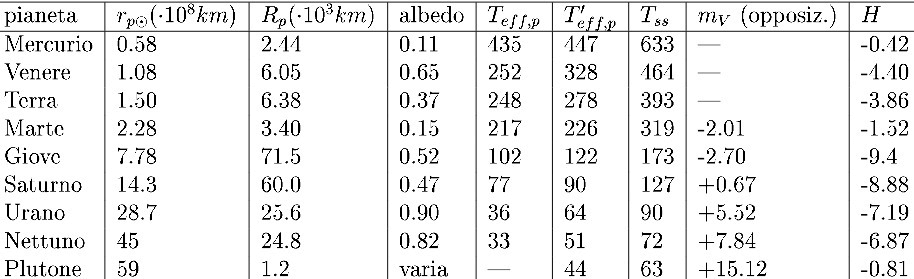
\includegraphics[width=(\textwidth),height=(0.9\textheight),keepaspectratio]{pianetiSS}
%\caption{Pianeti maggiori sistema solare.}
%\end{figure}



\subsection{Corpi minori.}

\begin{itemize}
    \item Satelliti
    \item Anelli
    \item Asteroidi, comete, TNO, ogetti della fascia di Kuiper-Edgeworth.
\end{itemize}

Forniscono informazioni sui processi di formazione del sistema solare.

\subsubsection{Evoluzione del sistema solare.}

Approccio statistico: processi collisionali e dinamici.

\subsubsection{Asteroidi.}

Orbite comprese tra Marte e Giove. Il primo \'e 1Ceres, diametro circa \SI{1000}{\kilo\meter}.

Da Terra si vedono come sorgenti puntiformi. Forma, dimensioni e caratteristiche superficiali: tecniche interferometriche e fenomeni di occultamento.

La spettro di riflessione \'e vario: dipende dalle caratteristiche chimiche e fisiche della superficie.

Sono la principale sorgente di meteoriti.

Classificazione in base a indici di colore (fotometria multibanda):
\begin{itemize}
    \item C: Condriti carbonacee.
    \item S: asteroidi con bassa albedo
\end{itemize}

Classificazione dinamica:
\begin{itemize}
    \item Fascia principale: tra Marte e Giove.
    \item Rapido spopolamento man mano che ci si avvicina a Giove.
    \item Lacune di Kirkwood: per valori del semi-asse maggiore risonanti con quello di Giove
    (Risonanza: rapporto periodo orbitale razionale non troppo distante da 1.).
    
    \begin{definition}{Risonanze orbitali}
    In celestial mechanics, an orbital resonance occurs when two orbiting bodies exert a regular, periodic gravitational influence on each other, usually due to their orbital periods being related by a ratio of two small integers. The physics principle behind orbital resonance is similar in concept to pushing a child on a swing, where the orbit and the swing both have a natural frequency, and the other body doing the "pushing" will act in periodic repetition to have a cumulative effect on the motion. Orbital resonances greatly enhance the mutual gravitational influence of the bodies, i.e., their ability to alter or constrain each other's orbits. In most cases, this results in an unstable interaction, in which the bodies exchange momentum and shift orbits until the resonance no longer exists. Under some circumstances, a resonant system can be stable and self-correcting, so that the bodies remain in resonance. Examples are the $1:2:4$ resonance of Jupiter's moons Ganymede, Europa and Io, and the $2:3$ resonance between Pluto and Neptune. Unstable resonances with Saturn's inner moons give rise to gaps in the rings of Saturn. The special case of 1:1 resonance (between bodies with similar orbital radii) causes large Solar System bodies to eject most other bodies sharing their orbits; this is part of the much more extensive process of clearing the neighbourhood, an effect that is used in the current definition of a planet.

A binary resonance ratio in this article should be interpreted as the ratio of number of orbits completed in the same time interval, rather than as the ratio of orbital periods, which would be the inverse ratio. Thus the 2:3 ratio above means Pluto completes two orbits in the time it takes Neptune to complete three. In the case of resonance relationships between three or more bodies, either type of ratio may be used (in such cases the smallest whole-integer ratio sequences are not necessarily reversals of each other) and the type of ratio will be specified.
    \end{definition}
\end{itemize}

\subsection{Tipi di risonanze orbitali}

In general, an orbital resonance may

    involve one or any combination of the orbit parameters (e.g. eccentricity versus semimajor axis, or eccentricity versus orbital inclination).
    act on any time scale from short term, commensurable with the orbit periods, to secular, measured in 104 to 106 years.
    lead to either long-term stabilization of the orbits or be the cause of their destabilization.

A mean-motion orbital resonance occurs when two bodies have periods of revolution that are a simple integer ratio of each other. Depending on the details, this can either stabilize or destabilize the orbit. Stabilization may occur when the two bodies move in such a synchronised fashion that they never closely approach. For instance:

    The orbits of Pluto and the plutinos are stable, despite crossing that of the much larger Neptune, because they are in a 2:3 resonance with it. The resonance ensures that, when they approach perihelion and Neptune's orbit, Neptune is consistently distant (averaging a quarter of its orbit away). Other (much more numerous) Neptune-crossing bodies that were not in resonance were ejected from that region by strong perturbations due to Neptune. There are also smaller but significant groups of resonant trans-Neptunian objects occupying the 1:1 (Neptune trojans), 3:5, 4:7, 1:2 (twotinos) and 2:5 resonances, among others, with respect to Neptune.
    In the asteroid belt beyond 3.5 AU from the Sun, the 3:2, 4:3 and 1:1 resonances with Jupiter are populated by clumps of asteroids (the Hilda family, the few Thule asteroids, and the extremely numerous Trojan asteroids, respectively).

Orbital resonances can also destabilize one of the orbits. For small bodies, destabilization is actually far more likely. For instance:

    In the asteroid belt within 3.5 AU from the Sun, the major mean-motion resonances with Jupiter are locations of gaps in the asteroid distribution, the Kirkwood gaps (most notably at the $3:1$, $5:2$, $7:3$ and $2:1$ resonances). Asteroids have been ejected from these almost empty lanes by repeated perturbations. However, there are still populations of asteroids temporarily present in or near these resonances. For example, asteroids of the Alinda family are in or close to the $3:1$ resonance, with their orbital eccentricity steadily increased by interactions with Jupiter until they eventually have a close encounter with an inner planet that ejects them from the resonance.
    In the rings of Saturn, the Cassini Division is a gap between the inner B Ring and the outer A Ring that has been cleared by a $2:1$ resonance with the moon Mimas. (More specifically, the site of the resonance is the Huygens Gap, which bounds the outer edge of the B Ring.)
    In the rings of Saturn, the Encke and Keeler gaps within the A Ring are cleared by 1:1 resonances with the embedded moonlets Pan and Daphnis, respectively. The A Ring's outer edge is maintained by a destabilizing $7:6$ resonance with the moon Janus.

Most bodies that are in resonance orbit in the same direction; however, a few retrograde damocloids have been found that are temporarily captured in mean-motion resonance with Jupiter or Saturn. Such orbital interactions are weaker than the corresponding interactions between bodies orbiting in the same direction.

A Laplace resonance is a three-body resonance with a 1:2:4 orbital period ratio (equivalent to a $4:2:1$ ratio of orbits). The term arose because Pierre-Simon Laplace discovered that such a resonance governed the motions of Jupiter's moons Io, Europa, and Ganymede. It is now also often applied to other 3-body resonances with the same ratios, such as that between the extrasolar planets Gliese 876 c, b, and e. Three-body resonances involving other simple integer ratios have been termed "Laplace-like" or "Laplace-type".

A Lindblad resonance drives spiral density waves both in galaxies (where stars are subject to forcing by the spiral arms themselves) and in Saturn's rings (where ring particles are subject to forcing by Saturn's moons).

A secular resonance occurs when the precession of two orbits is synchronised (usually a precession of the perihelion or ascending node). A small body in secular resonance with a much larger one (e.g. a planet) will precess at the same rate as the large body. Over long times (a million years, or so) a secular resonance will change the eccentricity and inclination of the small body.

Several prominent examples of secular resonance involve Saturn. A resonance between the precession of Saturn's rotational axis and that of Neptune's orbital axis (both of which have periods of about 1.87 million years) has been identified as the likely source of Saturn's large axial tilt ($26.7\deg$). Initially, Saturn probably had a tilt closer to that of Jupiter ($3.1\deg$). The gradual depletion of the Kuiper belt would have decreased the precession rate of Neptune's orbit; eventually, the frequencies matched, and Saturn's axial precession was captured into the spin-orbit resonance, leading to an increase in Saturn's obliquity. (The angular momentum of Neptune's orbit is 104 times that of Saturn's spin, and thus dominates the interaction.)

The perihelion secular resonance between asteroids and Saturn  helps shape the asteroid belt. Asteroids which approach it have their eccentricity slowly increased until they become Mars-crossers, at which point they are usually ejected from the asteroid belt by a close pass to Mars. This resonance forms the inner and "side" boundaries of the asteroid belt around 2 AU, and at inclinations of about $20\deg$.

Numerical simulations have suggested that the eventual formation of a perihelion secular resonance between Mercury and Jupiter has the potential to greatly increase Mercury's eccentricity and possibly destabilize the inner Solar System several billion years from now.

The Titan Ringlet within Saturn's C Ring represents another type of resonance in which the rate of apsidal precession of one orbit exactly matches the speed of revolution of another. The outer end of this eccentric ringlet always points towards Saturn's major moon Titan.

A Kozai resonance occurs when the inclination and eccentricity of a perturbed orbit oscillate synchronously (increasing eccentricity while decreasing inclination and vice versa). This resonance applies only to bodies on highly inclined orbits; as a consequence, such orbits tend to be unstable, since the growing eccentricity would result in small pericenters, typically leading to a collision or (for large moons) destruction by tidal forces.

In an example of another type of resonance involving orbital eccentricity, the eccentricities of Ganymede and Callisto vary with a common period of 181 years, although with opposite phases.

\subsubsection{Troiani.}

Sono oggetti che hanno lo stesso semi-asse di Giove ma spostati di \ang{+-60} nell'orbita cio\'e nei punti Lagrangiani.

\subsubsection{NEA/NEO.}

Orbita pi\'u interna, incrocia anche l'orbita della Terra.

\subsubsection{Comete.}
Orbite eccentriche.

Il cambiamento delle loro propriet\'a dipende dalla distanza dal Sole: ricche di sostanze volatili

Originaria di una fascia esterna di corpi minori compresa tra asteroidi e TNO, in seguito a incontri ravvicinati con corpi maggiori si sono spostate in orbite che raggiungono all'afelio i confini del sistema solare (Nube di Oort approx \SI{e5}{\astronomicalunit}: quando diventa prevalente l'attrazione delle stelle vicine).

\subsubsection{Centauri.}

Centauri: orbite comprese tra Giove e Nettuno. La zona \'e dinamicamente instabile e porta in orbite cometaria.

\subsubsection{Trans-Neptunian object: Fascia di Kuiper-Edgeworth.}

Oltre Nettuno di hanno i TNO.

Un sottogruppo dei TNO, i plutini, sono in risonanza $3:2$ con Nettuno (come Plutone).

\subsection{Search motivation}

\begin{itemize}
\item Why acretional formation of solar system planet objects should stop at Neptuno's distance.
\item The jupiter family comets are almost on planar orbits with low inclination on ecliptic plane (plane of solar system). This is inesplicable if the source is far away and isotropic, so we may may postulate a a disc of cometary object beyond Neptun.
\end{itemize}

\clearpage

\section{Interplanetary materials and meteorites}

\subsection{Comets}

\subsection{Asteroids}

\subsection{Short summary}
\begin{itemize}
\item Originate from primitive bodies: TNO, comets and asteroids.
\item Span 20 order of magnitude in mass
\item Observed ground or space based optically or IR: reflected solar light or thermal emission by small interplanetary dust arranged in a disk like structure on the ecliptic plane.
Zodiacal light is caused by reflected light at large angle, false corona light is attributed to small angle diffractive scattering.
\end{itemize}



\section{Grandezze caratteristiche del sole.}

\subsection{Et\'a del sole. Evolouzione pre-sequenza principale.}

\subsubsection{Datazione Meteoriti}

Per datare i meteoriti si usa il decadimento $^{87}Rb\to^{87}Sr$ con $\thalf=4.8\sci{10}\,yr$ o altri processi. La maggior parte dei meteoriti si sono formati nel disco di accrescimento ed hanno un'et\'a di $T=(4.55\pm0.05)\sci{9}\,yr$.


\subsubsection{Modello formazione sistema solare. Nascita proto-stella.}

\'E possibile mettere in relazione l'et\'a dei meteoriti con l'inizio della fase di sequenza principale del sole grazie ai modelli di formazione del sistema solare.
Il collasso di una nube di miglia di masse solari molto rarefatta \'e govarnato dal criterio di Jeans

\begin{equation}\label{eq:cjeans}
\frac{Gm(r)}{r}>\frac{RT}{\mu}
\end{equation}

In questo caso la nube si contrae con un tempo caratteristico $\tff=(\overline{\rho}G)\expy{-\frac{1}{2}}\approx\sci{7}\,yr$ e  il criterio di Jeans \'e verificato in sub-zone quindi la nube iniziale si  frammenta spontaneamente.

La materia del sottosistema che porter\'a alla formazione di una stella tipo Sole in seguito al collasso gravitazionale 

si addensa un core centrale in equilibrio idrostatico e il resto della materia forma un disco di accrescimento in free fall verso il core denso. Nel disco di accrescimento, per il tempo impiegato dalla disco a confluire sulla stella, ordine di $\sci{6}\,yr$, si sono formati la maggior parte dei meteoriti.~\ref{eq:cjeans}

\subsubsection{Inizio processi di fusione. Tempo in sequenza principale}

La luminosit\'a della protostella \'e alimentata dal collasso gravitazionale: dal teorema del viriale risulta che met\'a dell'energia gravitazionale guadagnata per unit\'a di tempo alimenta la luminosit\'a della proto-stella l'altra met\'a ne aumenta l'energia termica. Il tempo necessario perch\'e si raggiungano nella zona centrale densit\'a e temperature sufficienti per le reazioni di fusione \'e dell'ordine  del tempo-scala di \kh{}, $\tkh{}=\frac{Gm^2}{rL}$.


Il risultato della differenza tra l'et\'a del sistema solare e il tempo impiegato dal collasso a raggiungere le condizioni per la fusione dell'idrogeno \'e il periodo trascorso dal sole in sequenza principale:

L'et\'a del sole \'e $\tsun=(4.566\pm0.005)*\sci{9}\,yr$.
\begin{frame}{Giove}


\end{frame}

\begin{wordonframe}{giove}


\end{wordonframe}
